\chapter{ID Managing}

\section{Intro}

Il \textbf{furto di identità} si verifica quando qualcuno utilizza le informazioni
personali di identificazione di un'altra persona, come il nome, il numero di
identificazione o il numero di carta di credito, senza il suo permesso,
per commettere frodi o altri crimini.

\subsection{Identità digitale}

Un'\textbf{identità digitale} è un'informazione su un'entità utilizzata dai sistemi
informatici per rappresentare un agente esterno.
Tale agente può essere una persona, un'organizzazione, un'applicazione o un
dispositivo.
\textit{ISO/IEC 24760-1} definisce l'\textbf{identità} come
"insieme di attributi relativi a un'entità".
Le informazioni contenute in un'\textbf{identità digitale} consentono di valutare
e autenticare un utente che interagisce con un sistema aziendale sul web/Network,
senza il coinvolgimento di operatori umani.

\subsection{Autenticazione}

L'autenticazione è un aspetto fondamentale nella verifica dell'identità
di tipo \textbf{trust-based}, che consiste nel fornire un'assicurazione
dell'identità codificata tra un'identità e l'altra.
Le \textbf{metodologie di autenticazione} includono la presentazione di
un \textbf{oggetto univoco} come una carta di credito bancaria,
le \textbf{informazioni riservate} come una una password o la risposta a una
domanda prestabilita, \textbf{la conferma della proprietà di un indirizzo e-mail}.
Le soluzioni più robuste ma relativamente costose utilizzando metodologie di
crittografia.

\subsection{Autorizzazione}

L'autorizzazione è l'atto di controllare che un'entità abbia diritto ad
accedere ed utilizzare determinate risorse, essa
dipende dall'autenticazione, perché l'autorizzazione richiede
la verifica dell'attributo critico.

\section{Identity}

I concetti di \textbf{identità}, \textbf{identificatore} e \textbf{account} sono
strettamente correlati ma diversi.

\subsection{Identifier}

Il termine "\textbf{identificatore}" si riferisce a un singolo attributo il cui scopo
è quello di identificare in modo univoco una persona o un'entità,
all'interno di un contesto specifico. Alcuni esempi sono
indirizzo email, numero passaporto, ecc... .

\subsection{Identità}

Il termine "identità" è definito come un insieme di attributi associati a una
specifica persona/entità in un particolare contesto. Un'identità comprende uno o
più identificatori e può contenere altri attributi associati a una persona/entità.

\subsubsection{Attributi}

Le identità umane possono includere attributi come il nome, età, indirizzo,
numero di telefono, colore degli occhi e titolo di lavoro.
Le identità non umane possono includere attributi come il proprietario,
l'indirizzo IP e forse un numero di modello o di versione.
Gli attributi che compongono un'identità possono essere utilizzati per
l'autenticazione e l'autorizzazione, oltre che per trasmettere informazioni
sull'identità alle applicazioni.
Un'identità online consiste in almeno un identificatore e un insieme di attributi
per un utente/entità in un particolare contesto, come un'applicazione o una suite di
applicazioni.

\subsection{Account}

Un'identità è associata a un account in ciascuno di questi contesti.
Definiamo un account come un costrutto locale all'interno di una data
applicazione o suite di applicazioni che viene utilizzato per eseguire azioni
all'interno di quel contesto.
Gli attributi di identità possono essere contenuti in una struttura chiamata
account object all'interno di un'applicazione,
oppure possono essere memorizzati separatamente e referenziati dall'account object.

\subsection{Separazione tra ID e Account}

Un account può avere un proprio identificativo oltre a quello dell'identità ad
esso associata. Avere un identificatore dell'account separato dall'identità
associata all'account fornisce un grado di separazione.
L'identificativo dell'account può essere utilizzato in altri record dell'applicazione
per rendere più facile per gli utenti cambiare il nome utente o altro identificatore
associato al proprio account.
Si noti che un account può avere più di un'identità associata ad esso attraverso
l'account linking.

\subsection{Non Human Identifier}

Anche gli attori non umani possono certamente avere un'identità.
I componenti software che fungono da agenti o bot e i dispositivi intelligenti
possono avere un'identità e possono interagire con altri software o dispositivi
in modi che richiedono autenticazione e autorizzazione, proprio come gli attori
umani.

\subsection{IDM System}

Un Identity Management System(IdM) è un insieme di servizi che supportano
la creazione, la modifica e la rimozione delle identità e degli account associati
ad esse,
nonché l'autenticazione e l'autorizzazione necessarie per accedere alle risorse.
I sistemi di gestione dell'identità sono utilizzati per proteggere risorse online
da accessi non autorizzati e costituiscono un parte importante di un modello di
sicurezza completo.

\section{Eventi in un ciclo di vita di un'identità}

\begin{figure}[H]
    \centering
    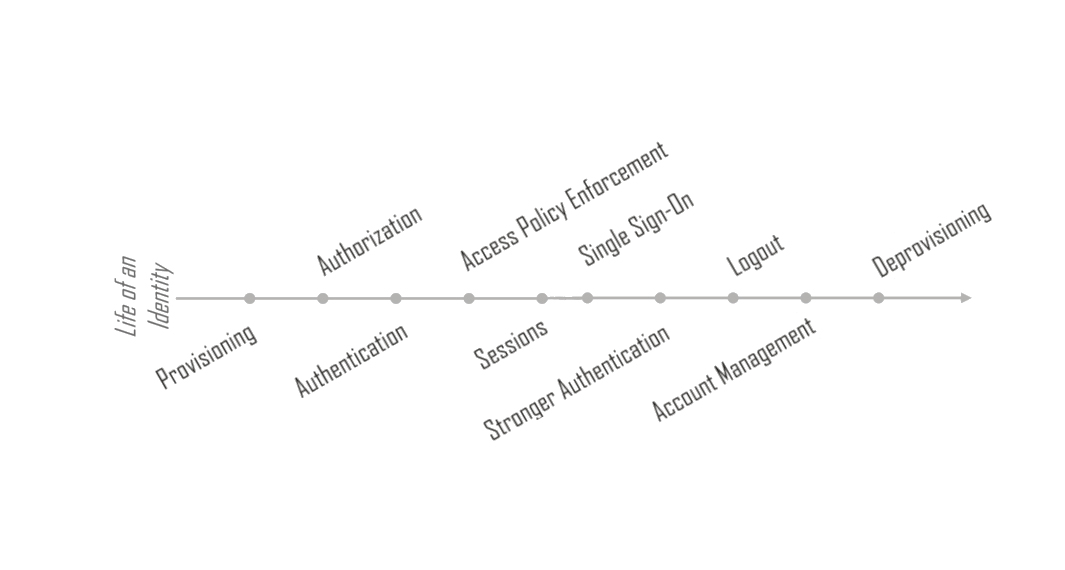
\includegraphics[width=\textwidth, keepaspectratio]{capitoli/id_managing/imgs/idman1.jpg}
\end{figure}

\subsection{PROVISIONING}

L'atto di creare un account e le relative informazioni di identità è spesso
indicato come provisioning.
L'obiettivo della fase di provisioning è quello di stabilire un account con i
relativi dati di identità.
Si tratta di ottenere o assegnare un identificativo univoco per l'identità,
opzionalmente un identificativo univoco per l'account distinto da quello
dell'identità, creare un account e associare gli attributi del profilo
dell'identità all'account.

\subsection{AUTHORIZATION}

Quando si crea un account, spesso è necessario specificare cosa può fare l'account,
sotto forma di privilegi.
Il termine autorizzazione indica la concessione di privilegi che regolano le attività
di un account.
L'autorizzazione di un account viene generalmente effettuata al momento della sua
creazione e può essere aggiornata nel tempo.

\subsection{AUTHENTICATION}

L'utente fornisce un identificativo per indicare l'account che desidera utilizzare e
inserisce le credenziali di accesso per l'account.
Queste vengono convalidate rispetto alle credenziali precedentemente registrate
durante la fase di provisioning dell'account.
Le credenziali possono riguardare qualcosa che l'utente conosce, qualcosa che
l'utente possiede e/o qualcosa che l'utente è.
Il nome utente indica l'account che l'utente desidera utilizzare e la conoscenza
della password dimostra il suo diritto a utilizzare l'account.

\subsection{ACCESS POLICY ENFORCEMENT}

%%TODO: ricontrollare tutto
L'autorizzazione specifica ciò che un utente o un'entità può fare. L'applicazione
dei criteri di accesso verifica che le azioni richieste da un utente siano
consentite dai privilegi che è stato autorizzato a utilizzare.

\subsection{SESSIONS}

Alcune applicazioni, in genere le applicazioni Web tradizionali e le applicazioni
sensibili, consentono a un utente di rimanere attivo solo per un periodo di tempo
limitato prima di richiedere all'utente di autenticarsi nuovamente.
(Una sessione tiene traccia delle informazioni)
Le impostazioni di timeout della sessione variano in genere in base alla
sensibilità dei dati dell'applicazione.

\subsection{SINGLE SIGN-ON}

Dopo aver effettuato l'accesso a un'applicazione, l'utente potrebbe voler
effettuare un'altra operazione con un'altra applicazione.
Il single sign-on (SSO) è la possibilità di effettuare il login una volta e poi
accedere ad altre risorse o applicazioni protette con gli stessi requisiti di
autenticazione, senza dover reinserire le credenziali.
Il single sign-on è possibile quando un insieme di applicazioni ha delegato
l'autenticazione alla stessa entità.

\subsection{STRONGER AUTHENTICATION}

L'autenticazione step-up è l'atto di elevare una sessione di autenticazione
esistente a un livello di garanzia più elevato mediante
autenticazione con una forma di autenticazione più forte.
Ad esempio, un utente potrebbe inizialmente accedere con un nome utente e una
password per stabilire una sessione di autenticazione.
In seguito, quando accede a una funzione o a un'applicazione più sensibile
con requisiti di autenticazione più elevati, all'utente vengono richieste
ulteriori credenziali, ad esempio una password una tantum generata sul suo
telefono cellulare.

\subsection{LOGOUT}

Come minimo, l'atto di disconnettersi dovrebbe terminare la sessione
dell'applicazione dell'utente.
Se l'utente ritorna all'applicazione, dovrà autenticarsi nuovamente prima di
poter accedere.
In situazioni in cui si utilizza il single sign-on, potrebbero esserci più
sessioni da terminare.
È una decisione di progettazione decidere quali sessioni debbano essere
terminare quando l'utente esce da un'applicazione.

\subsection{ACCOUNT MANAGEMENT AND RECOVERY}

Nel corso della vita di un'identità, può essere necessario modificare vari
attributi del profilo utente dell'identità.
Ad esempio, un utente potrebbe dover aggiornare il proprio indirizzo e-mail o
numero di telefono, la password e il nome.
In un'azienda, il profilo di un utente può essere aggiornato per riflettere una
nuova posizione, un nuovo indirizzo o nuovi privilegi come i ruoli.
Il recupero dell'account è un meccanismo per convalidare che un utente sia il
legittimo proprietario di un account attraverso alcuni mezzi secondari e quindi
consentire all'utente di stabilire nuove credenziali.
Ripristino della password smarrita via e-mail

\subsection{DEPROVISIONING}

Può capitare che sia necessario chiudere un account.
In questo caso, l'account dell'utente e le informazioni di identità associate
devono essere rimosse in modo che non possano più essere utilizzate.
Il deprovisioning può consistere nell'eliminazione completa dell'account e delle
informazioni di identità associate o nella semplice disabilitazione dell'account,
per conservare le informazioni a fini di revisione.